
\section{Methods of classification}\label{ch:methods}
There are countless possible ways in data science to classify data. The efficiency of methods varies in wide ranges for different types of problems.

In Sect. \ref{sec:basic} we learn about methods that are commonly used by data scientists. Following this, we discuss criteria for the choice of classifiers in Sect. \ref{sec:choice}. Based on this we present \emph{Logistic Regression} in Sect. \ref{sec:logReg} and \emph{k Nearest Neighbors} in Sect. \ref{sec:kNN} as our approaches to the challenge. This is followed by the winning submission by Gábor Melis in Sect. \ref{sec:win}. The chapter ends with Sect. \ref{sec:xgb}, presenting \emph{XGBoost} as winner of the \emph{HEP meets ML Award}.

\subsection{Basic data science methodology}\label{sec:basic}
Before we learn about criteria for choosing a good classification method, we present basic methods in data science. The performance of our approach can be influenced by the right use of these procedures.

\subsubsection{Feature selection and engineering}
An intuitive approach to optimize classifiers is to vary the used features of the data sets. The selection can be performed manually by considering e.g. histograms (Fig. \ref{fig:hist1}) , scatter plots (Fig. \ref{fig:scat1}), performance of various classifiers or automatically using techniques like PCA. Many automatic procedures tend to exclude features based on max errors, while the challenge aims to maximize AMS. Using such methods risks loosing important features\cite{blog}.

In the data, the value \emph{-999.0} is often set for certain features. This is a flag for \emph{missing} measurement in an event as sometimes a property simply cannot be measured, because fundamental effects do not happen.
The defining feature for missing values is \texttt{PRI\_jet\_num}, which is equal to the number of jets measured in a \emph{pp} collision. Given an event, where \texttt{PRI\_jet\_num} equals \emph{0}, there are 10 features that do not exist, only missing values in \texttt{DER\_mass\_MMC} are not related to this feature. The whole original dataset contains 567329 events with at least one feature missing, excluding missing \texttt{DER\_mass\_MMC}. This equals 70.9\% of all events and has to be considered for some classifiers. We bypass this problem by cutting these features for most methods. For simplicity, we only use the feature subsets presented in Tab. \ref{tab:feats} and the complete set of the original data.

\begin{table}
\begin{center}
\begin{minipage}{\textwidth}
	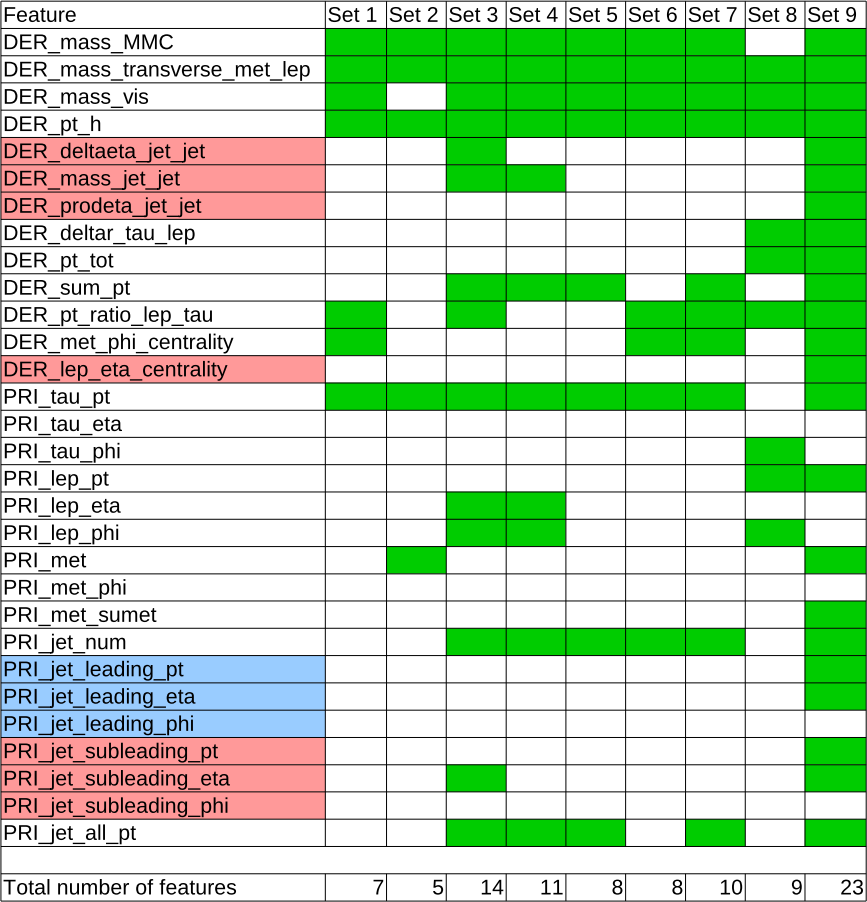
\includegraphics[width=\linewidth]{images/featsets}
	\vspace*{\baselineskip}
\end{minipage}
\begin{minipage}{.6\textwidth}
	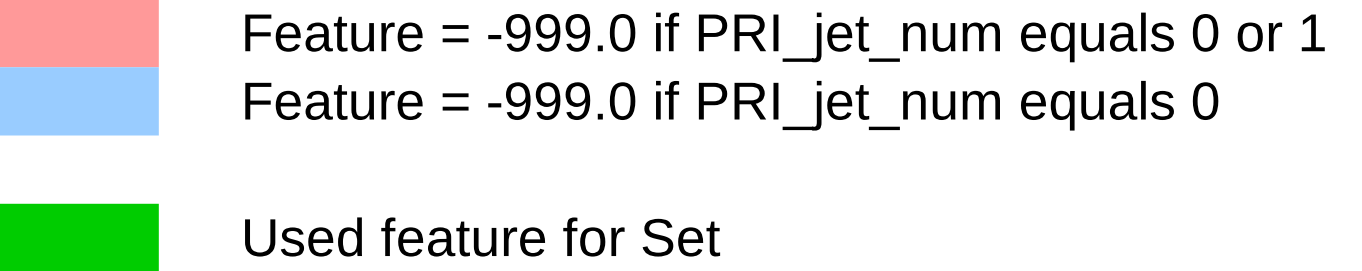
\includegraphics[width=\linewidth]{images/featsets-legend}
\end{minipage}
\hspace{1em}
\begin{minipage}{.35\textwidth}
	\caption{\\Feature subsets used by our approaches}
	\label{tab:feats}	
\end{minipage}
\end{center}
\end{table}

These sets are created before and during classification, latter as part of optimization efforts. Sets 1 and 2 are chosen beforehand as result of the visualization of the features, e.g. \texttt{DER\_mass\_MMC} seems to be well separable, so it is added to most sets although it has missing values. Sets 3,4 and 5 result of an ensemble of 50 \emph{k Nearest Neighbors} classifiers, which will be described in Sect. \ref{sec:kNN}, each choosing 5 random features. These sets contain a number of the common features used for the best predictions generated by this ensemble. The Sets 6 and 7 are chosen by hand to improve \emph{k Nearest Neighbors}. Set 8 results of an ensemble of \emph{Logistic Regression} classifiers (Sect. \ref{sec:logReg}). Like before, we choose the common features used for the best predictions of the ensemble. Set 9 is the only feature set suggested by a competitor in the challenge \cite{blog}.

Because of its origin in physics, the calculation of more topic-relevant features seems as a promising use of domain-knowledge. However, the top-participants of the challenge shared the observation that artificial features did not improve the AMS significantly \cite{melis-1st,salimans-2nd,courtiol-3rd}.

\subsubsection{Cross-validation}
Overfitting a model is a known problem in machine learning. In the leaderboards we can observe single submissions to the challenge that had big differences in ranks on the public and private leaderboard. This could be explained by overfitted classifiers, in one case a submission fell 720 ranks from its public to private rank. \\
A common technique to prevent overfitting is to use only one part of the training set for fitting the classifier while using the other one for testing, calculating a evaluation score, like \emph{mean squared error} (MSE). This method is called \emph{cross-validation}.  Multiple contestants stated, that simple cross-validation is not able to reliably estimate the submission's AMS. A solution to this is to repeat this procedure with different splits of the training data, which increases the runtime of the estimation by cross-validation.

\subsection{Choosing the classifiers}\label{sec:choice}
In order to choose an effective approach to a solution for the challenges task, we need to consider several dependencies of a classifier.

\subsubsection{Computational resources}
One basic limitation of our choice are the available resources.
We want our classification to efficiently use the system represented by Tab. \ref{tab:specs}.

\begin{SCtable}[1][h]
  	\begin{tabular}{r l||}
		Operating System: & Windows 8.1 64bit\\
		CPU: & Intel i7 K875 @ 2.93GHz (4 Cores)\\
		Memory: & 16GB DDR3\\
		GPU: & NVIDIA GeForce GTX470 @ 1.22GHz\\
		VRAM: & 1280 MB GDDR5\\
	\end{tabular}
	\caption{\\Specifications of used System}
	\label{tab:specs}
\end{SCtable}

While this hardware enables us to use various methods that utilize minor  parallelization, it still limits the performance of classifiers dependent on high parallelization, like neural networks. If not stated differently, all presented data on \emph{runtime} in this thesis is based on the system represented by Tab. \ref{tab:specs}.

\subsubsection{Dependency on data}
The choice of classifiers is dependent on the amount of data. The training set contains 250000 samples with 32 features (EventId not counted), the test set 550000 samples with 30 features. Considering this, some classification methods would be ineffective, e.g. the implementation of \emph{Support Vector Classification} in scikit-learn, which is quadratic in the number of examples \cite{sklearn}.

\subsubsection{scikit-learn}
For the approaches we implemented, we will version 0.17 of \emph{scikit-learn}, an open source machine learning library for Python. Originated from a "Google Summer of Code" project started 2007, it grew into a popular toolkit \cite{sklearn}.
Using scikit-learn has advantages and disadvantages, Tab. \ref{tab:sklearn} considers the most important ones.

\begin{table}[h]
\begin{center}
	\begin{tabular}{ | p{0.3\textwidth} | p{0.65\textwidth} |}
  		\hline
		\multicolumn{2}{ |c| }{Advantages} \\
		\hline
		Usability &
		Scikit-learn is easily installed via Python-package manager systems like \emph{pip} or \emph{Anaconda}, its required dependencies are NumPy, SciPy, and a working C/C++ compiler\cite{sklearngit}. It is compatible with Windows 8.1 64bit.\\
		\hline
		Scale and documentation &
		A reason for its popularity is the amount of common algorithms this toolkit contains. It also offers good code-documentation and mathematical explanation of all models included.\\
		\hline
		Multi-core CPU support &
		With every version, scikit-learn improves its multi-core support for algorithms that profit of parallelization\cite{sklearnhistory}. This will speed up our classification considerably.\\
		\hline
		\hline
		\multicolumn{2}{ |c| }{Disadvantages} \\
		\hline
		No GPU support: &
		While the library utilizes multi-core CPUs, GPU-parallelization is not supported by scikit learn.\\
		\hline
		(Almost) no custom \newline scoring functions &
		Scikit-learn offers rarely an easy way to use custom evaluation functions for e.g. fitting a classifier. Some algorithms, like \emph{sklearn.cross\_validation}, offer a choice of pre-built functions via a \emph{scoring} parameter.\\
		\hline
		Speed &
		One focus of the development of the toolkit is to optimize and speed up the algorithms, but projects devoted to single learning techniques are probably faster.\\
		\hline
	\end{tabular}
	\caption{Comparison of scikit-learn's properties}
	\label{tab:sklearn}
	\end{center}
\end{table}

Sect. \ref{sec:logReg} and \ref{sec:kNN} describe our approach. Information regarding the source code is found in Appendix \ref{app:code}.

\begin{itemize}
	\item optimizing objective function
	\item AMS
\end{itemize}

\begin{itemize}
	\item why kNN?
	\item what is kNN?
	\item optimization
	\item performance
	\item AMS
	\item \cite{californiaPaper} are noobs :-P
\end{itemize}

\subsection{The winning submission}\label{sec:win}
The three top submissions of the challenge all use classification methods that rely heavily on strong hardware. Without the ability to recreate these submissions or use various parameter changes, we focus solely on understanding the winning model, relying on \cite{meli14}.

\subsubsection{Neural Networks in general}
A \emph{neural network} is a type of machine learning model that was inspired by central nervous systems, like the human brain. Blocks or \emph{neurons} are basic mathematical operations, like simple linear or bias functions. These neurons are grouped into so-called \emph{layers}, which can be interpreted as weighting functions. The weights are optimized via loss functions, like \emph{Squared Error}, during the training phase of this learning model. Usually neural networks have an \emph{input layer}, a number of \emph{hidden layers} and an \emph{output layer}. A user or an external algorithm can only interact through the input layer, delivering data to the network, and the output layer, receiving an estimation on this data.\\
A neural network is fitted with so-called \emph{backpropagation}. To understand this procedure, we use a mathematical expression of neural networks with one hidden layer, following  \cite{harmeling18}:

\begin{eqnarray}\label{eqn:nn}
\begin{tabular}{r l l}
		&$z_1 = x$ & input layer\\
		&$z_2 = f_1(w_1,z_1)$ & second layer (hidden)\\
		$y =$&$z_3 = f_2(w_2,z_2)$ & output layer\\ \\
		&$E = \frac{1}{2}(y-t)^2$ & squared error (loss function) \hspace{1em},
\end{tabular}
\end{eqnarray}

where $f_1$ and $f_2$ are a differentiable functions. While the weight  $w_1$ and the value $z_1$ are input of $f_1$, $z_2$ is its output. Analogous, $f_2$ produces the networks output, using $w_2$ and $z_2$. $E$ is a loss function, here \emph{squared error}.\\
The output of a layer is highly dependent on this layers input. Therefore, changing a weight of a previous layer influences all following layers. If we differentiate the loss function $E$ w.r.t. $w_1$ by applying the chain rule, we can observe its connection to following layers.

\begin{equation}\label{eqn:nn_der}
\frac{\partial E}{\partial w_1} = \frac{\partial E}{\partial z_3} \frac{\partial z_3}{\partial z_2} \frac{\partial z_2}{\partial w_1}
\end{equation}

Backpropagation uses this connection and tunes the weights of each neuron of each layer. For instance, the layer $f_2$ receives the loss function derivative w.r.t. this layers output, i.e. $\frac{\partial E}{\partial z_3}$. It calculates the resulting derivation of $E$ w.r.t. $w_2$:
\begin{equation}\label{eq:nn_Ew2}
	\frac{\partial E}{\partial w_2} = \frac{\partial E}{\partial z_3} \frac{\partial}{\partial w_2} f_2(w_2,z_2)
\end{equation}

The layer uses $\frac{\partial E}{\partial w_2}$ to update the weights with \emph{gradient descent} at a sometimes automatically chosen regularization strength $\eta$. The weight approaches an optimal value with respect to the loss function.

In practice, the derivation for each layer is known and stored in the code, we only recalculate values resulting from these functions. The ability to highly parallelize backpropagation by using GPUs is the reason for its increasing popularity during the last years.

\subsubsection{The method}
The model developed by Gábor Melis uses an ensemble of 70 neural networks with three hidden layers containing 600 neurons each. The output layer consists of two \emph{softmax} units, which basically normalize the weight-combinations to get a prediction for each class.
Each neural network is fitted by a different split of the training data that is normalized to mean 0 and variance 1 and different weight-initializations. The hidden layers utilize \emph{Local Winner-Take-All activation}, which cancel all weighted input values received by three blocks except for the maximum. The weighting is optimized with respect to a cross-entropy objective function using backpropagation with stochastic gradient descent.
The winning submission, which has been generated by this classifier, outperforms follow-up submissions by over 0.015 AMS. It uses artificial features and was created within a runtime of 10 minutes on a GTX Titan GPU \cite{meli14}.

\subsection{XGBoost}\label{sec:xgb}
One noteworthy classification method is \emph{Gradient Boosting} and its implementation by Tianqi Chen and Tong Hel via the package \emph{XGBoost}.
After sharing it with other participants early in the challenge, they were rewarded with a special jury-award, for providing "a good compromise between performance and simplicity"\cite{HEPml}. While describing XGBoost, we evaluate this method by these criteria.
For our testing, we use the python package of XGBoost version 0.47 available at \url{https://github.com/dmlc/xgboost}, released on 15. Jan. 2016.

\subsubsection{Boosting}
Assuming, we fit a model to solve a problem. A classifier is called a \emph{strong learner} if it performs well and its prediction achieves a high accuracy. Therefore, a \emph{weak learner} is a classifier that performs poorly, but learns from a training set, the prediction is not made by random guessing.
\emph{Boosting} is the idea to combine a set of weak learners into a single strong learner.

Given training data $x$ with true label $y$, we fit a weak learner $f_1(x)$, which predicts the label $\hat{y}$.
\begin{equation}\label{eq:boosting1}
	y = f_1(x) + z \mathrm{\hspace{1em} ,}
\end{equation}
where $z$ is the prediction error $|y-\hat{y}|$.\\
We replace the error with a second classifier in Eq. \eqref{eq:boosting1} such that
\begin{equation}\label{eq:boosting2}
	y = f_1(x) + f_2(x) \mathrm{\hspace{1em},}
\end{equation}
or equivalently
\begin{equation}\label{eq:boosting3}
	f_2(x) = y - f_1(x) \mathrm{\hspace{1em}.}
\end{equation}
Considering we create an ensemble of weak learners, $f_2$ will not correct $f_1$'s prediction perfectly. To approximate a good \emph{fix} we fit $f_2$ not to the training data $x$, but to the error $y - f_1(x)$, the so-called \emph{residual}.\\
In words: Because our solution is not perfect, we expect an error in our prediction. Therefore, we train another model to fit this error and repeat this process a set number of times.

\subsubsection{Classification method}
Boosting can be trained by minimizing an objective function
\begin{equation}\label{eq:boost_objective}
	L = \sum\limits_{j=1} l ( y_j,F(x_j)) \mathrm{\hspace{1em},}
\end{equation}
where \emph{l} is a loss function, $y_j$ the \emph{true} label of $x_j$ and $F$ is an ensemble of weak learners $\{f_1,f_2,\ldots,f_n\}$. If we use \emph{square loss} as loss function $l$ and differentiate this w.r.t. a weak learner $f_1(x_j)$ of the ensemble such that
\begin{equation}\label{eq:boostloss}
	\frac{\partial l}{\partial f_2(x_j)} = y - f_1(x_j) \mathrm{\hspace{1em},}
\end{equation}
we can observe that $- \frac{\partial l}{\partial f_2(x_j)}$ equals the residual $f_2(x) = y - f_1(x)$.
Thus, residuals of a Boosting model can be interpreted as negative \emph{gradients} that allows minimization of the loss function using \emph{gradient descent}. This is called \emph{gradient boosting}. Further, one can show that a gradient boosting algorithm can be constructed for \emph{any} loss function \cite{gradboost}.

The more complex a classification model is, the higher is the chance of overfitting. Considering this, the main difference of XGBoost to other gradient boosting classifiers is the simple idea to penalize complex models in the ensemble. This is achieved by adding a regularization term $\Omega(f)$, which measures the complexity of $f$, to the objective function Eq.\eqref{eq:boost_objective}. Training this classifier minimizes not only the loss function, but also $\Omega(f_t)$.
The actual predictions are made by weighted \emph{decision trees} with a chosen maximum depth, which are initialized with random values.

We visualize a tree in Fig. \ref{fig:tree} using XGBoost's \emph{plot\_tree} method. It is one of 100 trees fitted to the original training data with a maximum depth of 3.
\begin{figure}[h]
\begin{center}
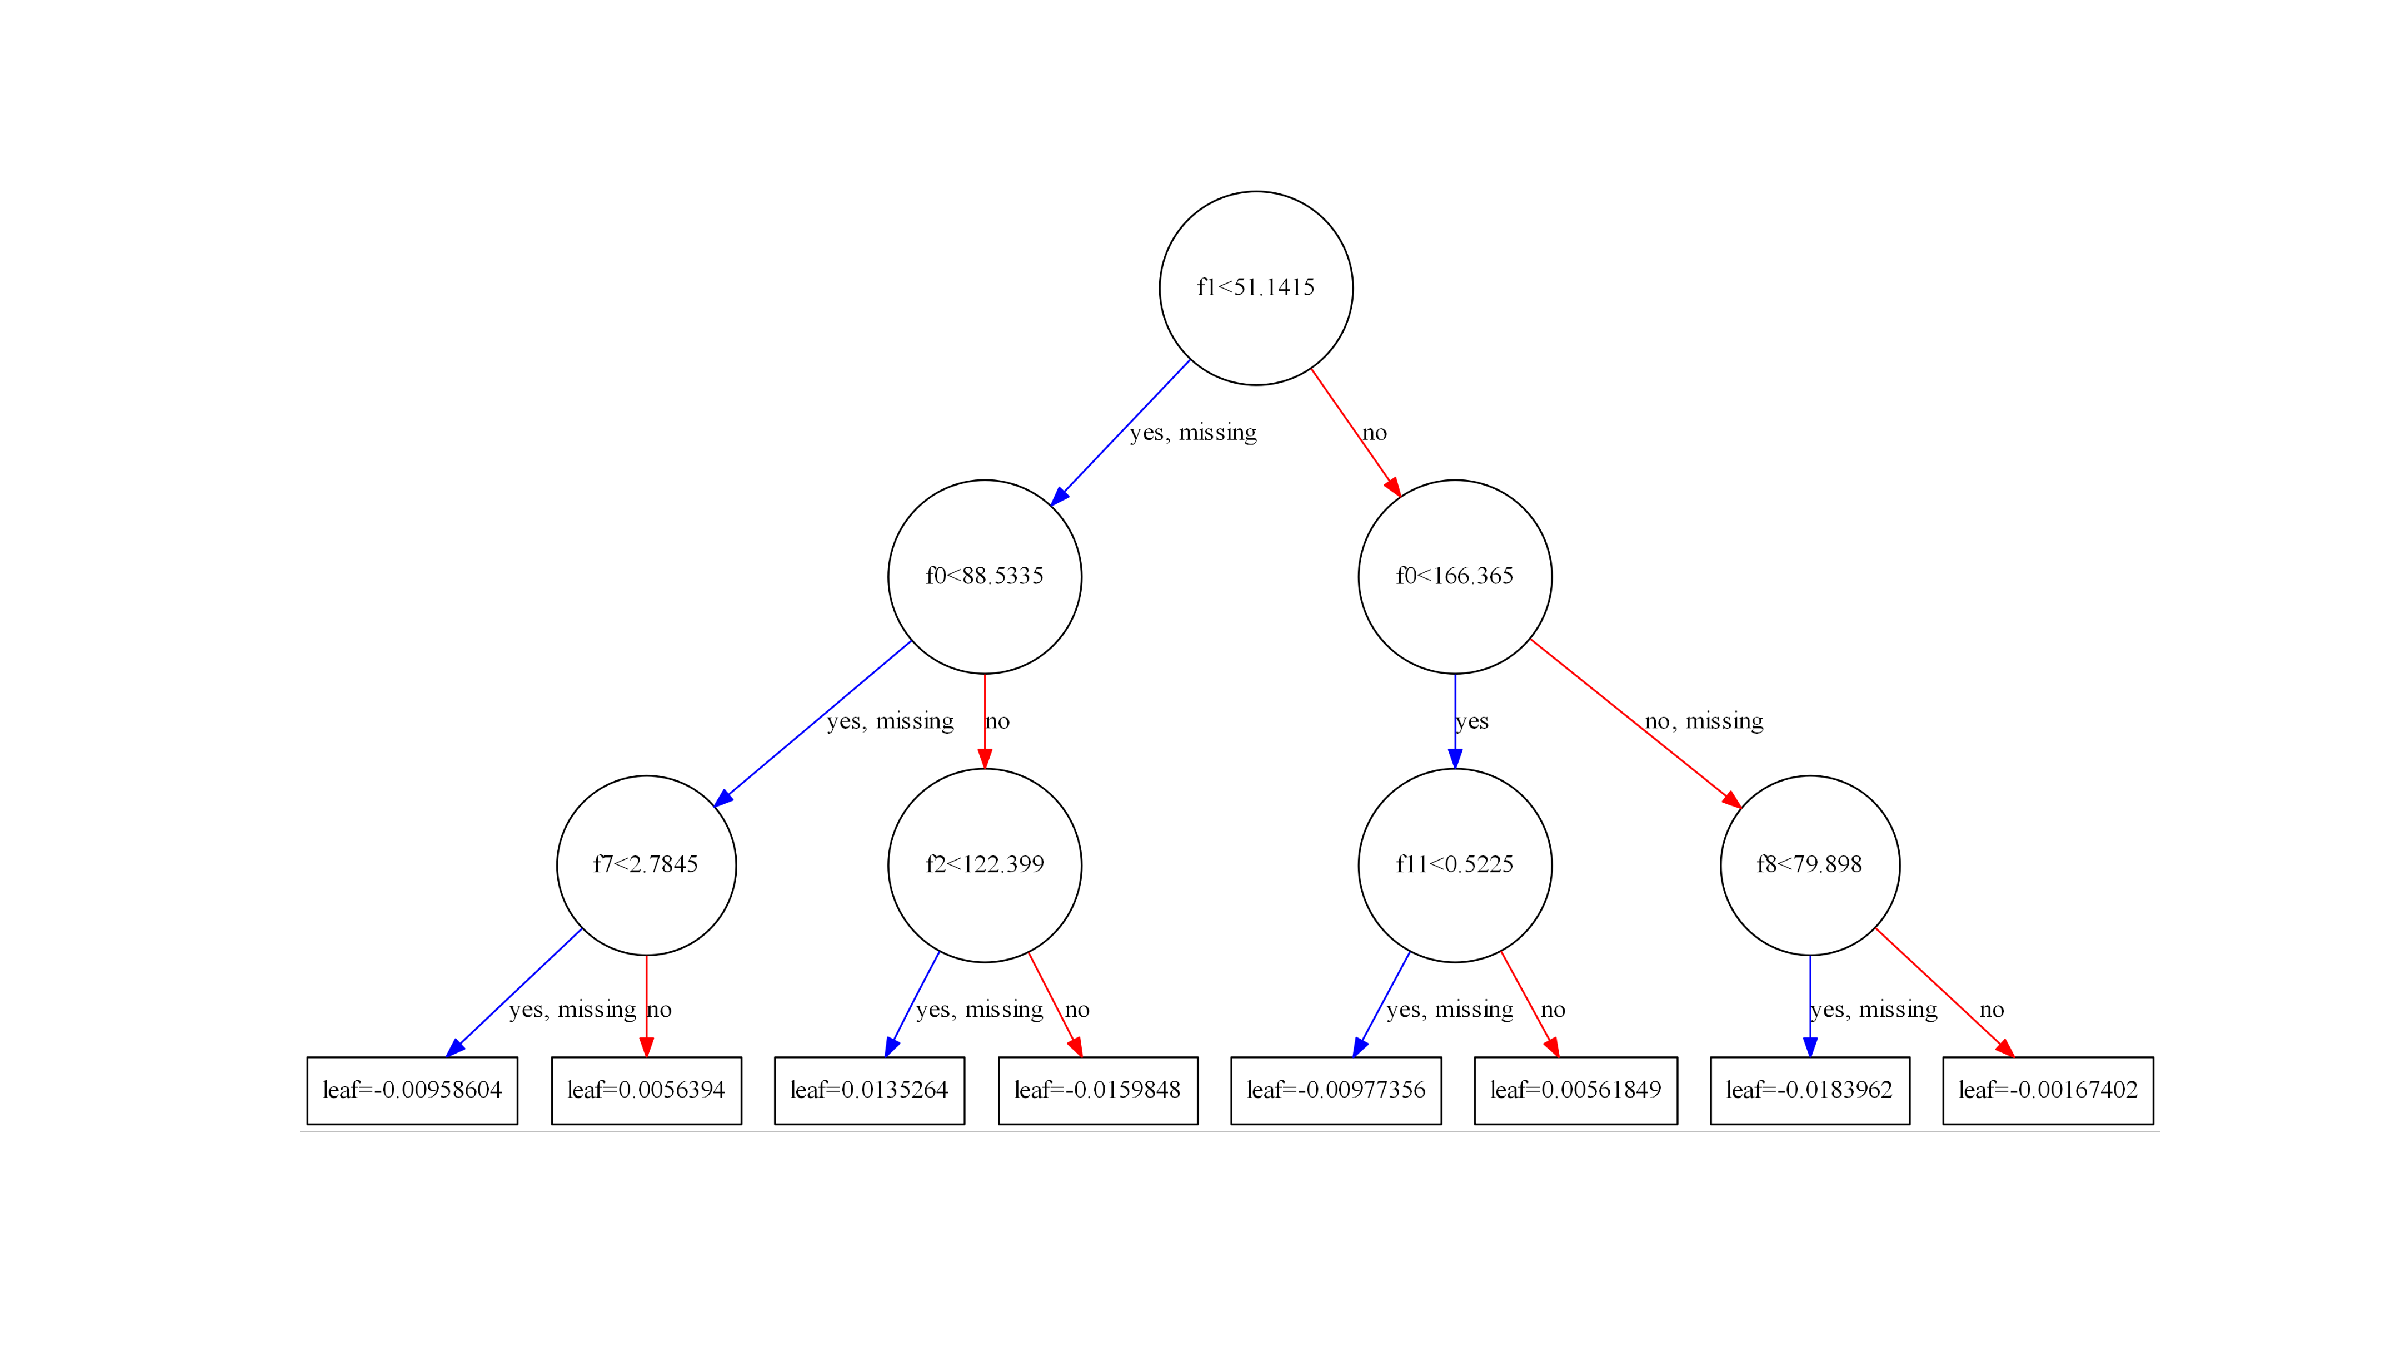
\includegraphics[trim=146 100 118 90, clip, width=\textwidth]{images/tree.pdf}
\caption{A decision tree generated by XGBoost.}
\label{fig:tree}
\end{center}
\end{figure}
\subsubsection{Performance and optimization}
Using default settings, 100 trees and AMS evaluation, XGBoost achieves a public AMS of about 3.32 using the complete, original data set. We get significantly better results by tuning parameters with respect to the public AMS, mainly increasing the number of trees up to 3000 and lowering \emph{eta}. Latter parameter determines the \emph{step size shrinkage} to prevent overfitting. Testing shows that \emph{eta} is inversely related to the tree number, the more trees are used for training, the lower should \emph{eta} be chosen.
Using all parameters, we are still not able to reproduce the exact AMS on the original data stated in \cite{chen14}.
Cutting phi-values, which is suggested by some competitors that use XGBoost \cite{blog}, does not improve the results. Further feature selection fails to resolve into better AMS. Adding artificial features works beneficial for several submissions using the method.\\
In its recent version, XGBoost provides several alternative objective functions and evaluation metrics. As the package has been developed for the Kaggle challenge, it also contains AMS and AUC as metrics. While the original submission used AUC as model evalutation, we use AUC \emph{and} AMS for training XGBoost with no noticeable disadvantages.

Many software packages implement gradient boosting, as it is an established method in machine learning. While Fig. \ref{fig:xgb-speed} compares speed benchmarks, with all algorithms set up to fit 120 trees with depth 6 and \emph{eta}=0.1, we consider AMS as it is the main goal of the challenge. Since our approaches rely on scikit-learn, we compare the performance of the \emph{GradientBoostingClassifier}(GBC) class to XGBoost , see Fig. \ref{fig:xgb-gbc}.\\
The training GBC consumes over 5000 seconds, while using 100 trees of depth 12. Considering the long training time, we do not perform further training of GBC with more trees. However, it is worth mentioning that the longest training, that was performed on a XGBoost classifier for this thesis, terminated after 1666 seconds, calculating 3000 trees with a depth of 12.
By preprocessing the mathematical model and using decision trees, the training complexity for a tree is reduced to $O(ndK)$ for \emph{n} samples with \emph{d} features, where \emph{K} is the maximum depth of a decision tree\cite{chen14}.

\begin{figure}[h]
\centering
\begin{minipage}[b]{0.48\textwidth}
  \centering
  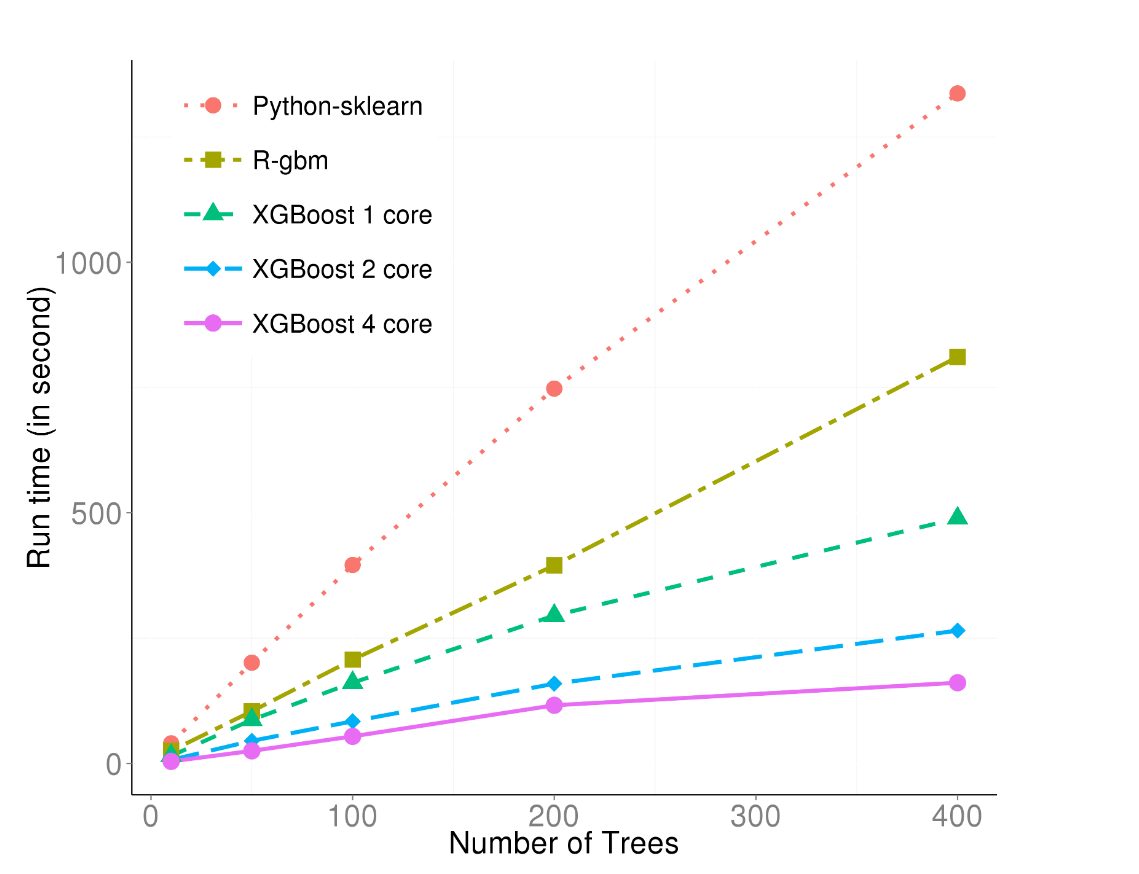
\includegraphics[trim=0 14 60 0,clip,width=\linewidth]{images/xgboost-speed}
  \vspace{-0.1ex}
	\caption{Speed Benchmark on challenge data \cite{chen14}}
	\label{fig:xgb-speed}
\end{minipage}
\quad
\begin{minipage}[b]{0.48\textwidth}
  \centering
  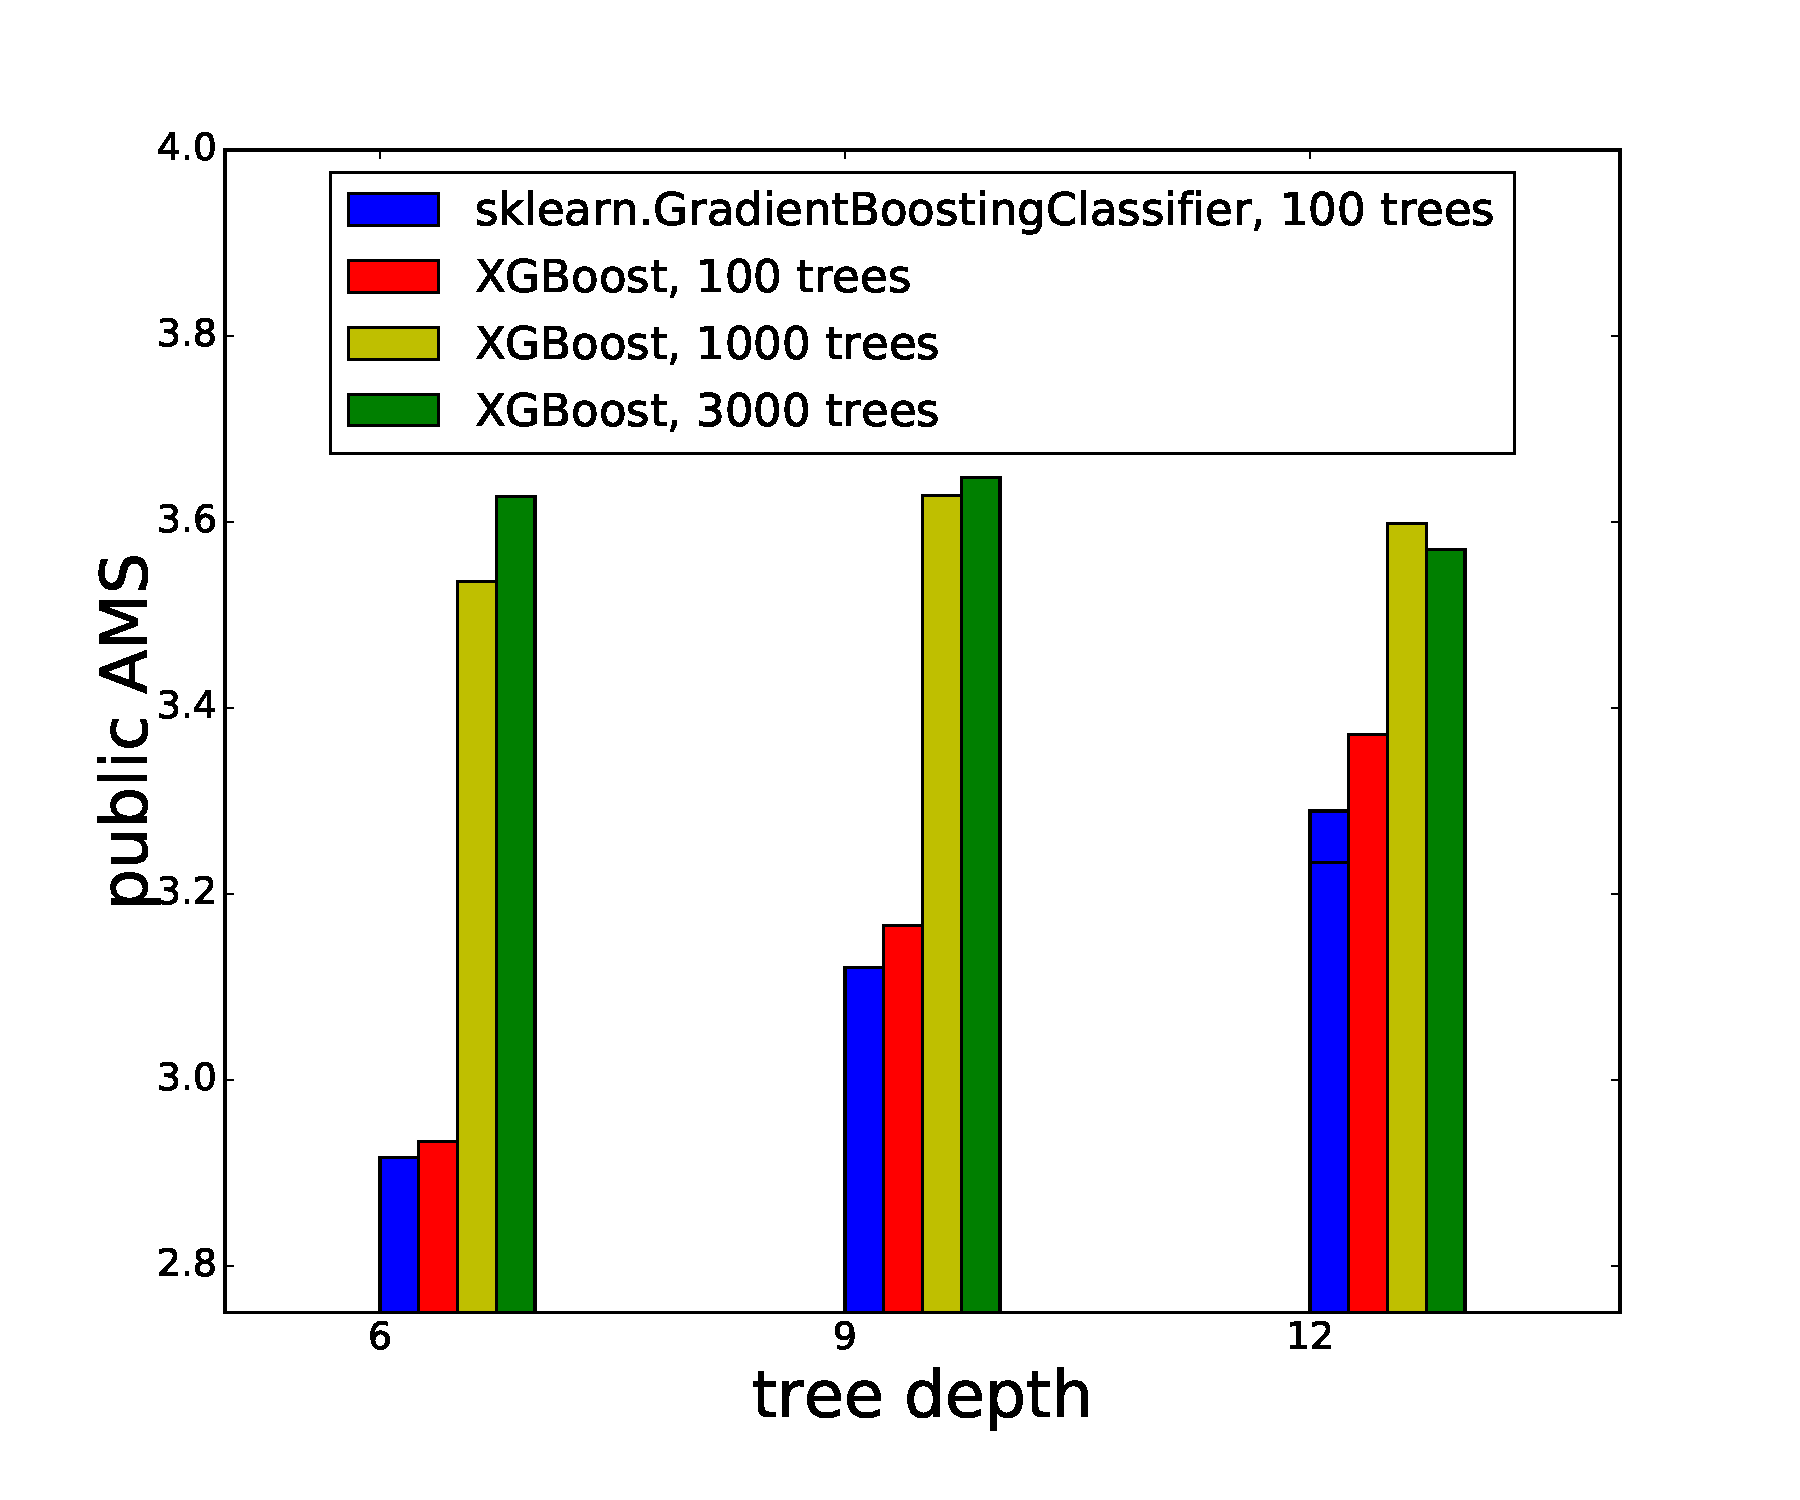
\includegraphics[trim=30 0 40 0,clip,width=\linewidth]{images/xgb-gbc.pdf}
	\caption{AMS-Comparison XGBoost and sklearn.GradientBoostingClassifier}
	\label{fig:xgb-gbc}
\end{minipage}
%\vspace{1ex}
\end{figure}

Regarding the special award, XGBoost seems to fulfil every of its defined aspects. While many other submissions outperform the best benchmark \emph{MultiBoost} easily as well, this package does it remarkably fast. Training time for a benchmark surpassing result takes under 37 seconds with tuned parameters, using up to 8 CPU threads. This specific run achieved a public AMS of 3.5399.
The developers made the package available early in the challenge and many other participants used it at some point to test custom feature sets or benchmark their own approaches.

It is justified to acknowledge this package, as it could have impact on tools, which are being used in high energy physics\cite{HEPml}.

\pagebreak

%%%%%%%%%%%%%%%%%%%%%%%%%%%%%%%%%%%%%%%%%%%%%%%%%%%%%%%%%%%%%%%%%%%%%
% Leerseite bei zweiseitigem Druck
%%%%%%%%%%%%%%%%%%%%%%%%%%%%%%%%%%%%%%%%%%%%%%%%%%%%%%%%%%%%%%%%%%%%%
\ifthenelse{ \( \equal{\zweiseitig}{twoside} \and \not \isodd{\value{page}} \)}
	{\pagebreak \thispagestyle{empty} \cleardoublepage}{\clearpage}